%!TEX TS-program = xelatex

% Шаблон документа LaTeX создан в 2018 году
% Алексеем Подчезерцевым
% В качестве исходных использованы шаблоны
% 	Данилом Фёдоровых (danil@fedorovykh.ru) 
%		https://www.writelatex.com/coursera/latex/5.2.2
%	LaTeX-шаблон для русской кандидатской диссертации и её автореферата.
%		https://github.com/AndreyAkinshin/Russian-Phd-LaTeX-Dissertation-Template

\documentclass[a4paper,14pt]{article}

%%% Работа с русским языком
\usepackage[english,russian]{babel}   %% загружает пакет многоязыковой вёрстки
\usepackage{fontspec}      %% подготавливает загрузку шрифтов Open Type, True Type и др.
\defaultfontfeatures{Ligatures={TeX},Renderer=Basic}  %% свойства шрифтов по умолчанию
\setmainfont[Ligatures={TeX,Historic}]{Times New Roman} %% задаёт основной шрифт документа
\setsansfont{Comic Sans MS}                    %% задаёт шрифт без засечек
\setmonofont{Courier New}
\usepackage{indentfirst}
\frenchspacing

\renewcommand{\epsilon}{\ensuremath{\varepsilon}}
\renewcommand{\phi}{\ensuremath{\varphi}}
\renewcommand{\kappa}{\ensuremath{\varkappa}}
\renewcommand{\le}{\ensuremath{\leqslant}}
\renewcommand{\leq}{\ensuremath{\leqslant}}
\renewcommand{\ge}{\ensuremath{\geqslant}}
\renewcommand{\geq}{\ensuremath{\geqslant}}
\renewcommand{\emptyset}{\varnothing}

%%% Дополнительная работа с математикой
\usepackage{amsmath,amsfonts,amssymb,amsthm,mathtools} % AMS
\usepackage{icomma} % "Умная" запятая: $0,2$ --- число, $0, 2$ --- перечисление

%% Номера формул
%\mathtoolsset{showonlyrefs=true} % Показывать номера только у тех формул, на которые есть \eqref{} в тексте.
%\usepackage{leqno} % Нумерация формул слева	

%% Перенос знаков в формулах (по Львовскому)
\newcommand*{\hm}[1]{#1\nobreak\discretionary{}
	{\hbox{$\mathsurround=0pt #1$}}{}}

%%% Работа с картинками
\usepackage{graphicx}  % Для вставки рисунков
\graphicspath{{images/}}  % папки с картинками
\setlength\fboxsep{3pt} % Отступ рамки \fbox{} от рисунка
\setlength\fboxrule{1pt} % Толщина линий рамки \fbox{}
\usepackage{wrapfig} % Обтекание рисунков текстом

%%% Работа с таблицами
\usepackage{array,tabularx,tabulary,booktabs} % Дополнительная работа с таблицами
\usepackage{longtable}  % Длинные таблицы
\usepackage{multirow} % Слияние строк в таблице
\usepackage{float}% http://ctan.org/pkg/float

%%% Программирование
\usepackage{etoolbox} % логические операторы


%%% Страница
\usepackage{extsizes} % Возможность сделать 14-й шрифт
\usepackage{geometry} % Простой способ задавать поля
\geometry{top=20mm}
\geometry{bottom=20mm}
\geometry{left=20mm}
\geometry{right=10mm}
%
%\usepackage{fancyhdr} % Колонтитулы
% 	\pagestyle{fancy}
%\renewcommand{\headrulewidth}{0pt}  % Толщина линейки, отчеркивающей верхний колонтитул
% 	\lfoot{Нижний левый}
% 	\rfoot{Нижний правый}
% 	\rhead{Верхний правый}
% 	\chead{Верхний в центре}
% 	\lhead{Верхний левый}
%	\cfoot{Нижний в центре} % По умолчанию здесь номер страницы

\usepackage{setspace} % Интерлиньяж
\onehalfspacing % Интерлиньяж 1.5
%\doublespacing % Интерлиньяж 2
%\singlespacing % Интерлиньяж 1

\usepackage{lastpage} % Узнать, сколько всего страниц в документе.

\usepackage{soul} % Модификаторы начертания

\usepackage{hyperref}
\usepackage[usenames,dvipsnames,svgnames,table,rgb]{xcolor}
\hypersetup{				% Гиперссылки
	unicode=true,           % русские буквы в раздела PDF
	pdftitle={Автоматизация проектных работ},   % Заголовок
	pdfauthor={Солодянкин А.А.},      % Автор
	pdfsubject={Автоматизация проектных работ},      % Тема
	pdfcreator={Солодянкин А.А.}, % Создатель
	pdfproducer={Солодянкин А.А.}, % Производитель
	pdfkeywords={Автоматизация проектных работ}, % Ключевые слова
	colorlinks=true,       	% false: ссылки в рамках; true: цветные ссылки
	linkcolor=black,          % внутренние ссылки
	citecolor=black,        % на библиографию
	filecolor=magenta,      % на файлы
	urlcolor=black           % на URL
}
\makeatletter 
\def\@biblabel#1{#1. } 
\makeatother
\usepackage{cite} % Работа с библиографией
%\usepackage[superscript]{cite} % Ссылки в верхних индексах
%\usepackage[nocompress]{cite} % 
\usepackage{csquotes} % Еще инструменты для ссылок

\usepackage{multicol} % Несколько колонок

\usepackage{tikz} % Работа с графикой
\usepackage{pgfplots}
\usepackage{pgfplotstable}

% ГОСТ заголовки
\usepackage[font=small]{caption}
%\captionsetup[table]{justification=centering, labelsep = newline} % Таблицы по правобу краю
%\captionsetup[figure]{justification=centering} % Картинки по центру


\newcommand{\tablecaption}[1]{\addtocounter{table}{1}\small \begin{flushright}\tablename \ \thetable\end{flushright}%	
\begin{center}#1\end{center}}

\newcommand{\imref}[1]{рис.~\ref{#1}}

\usepackage{multirow}
\usepackage{spreadtab}
\newcolumntype{K}[1]{@{}>{\centering\arraybackslash}p{#1cm}@{}}


\usepackage{xparse}
\usepackage{fancyvrb}

\RecustomVerbatimCommand{\VerbatimInput}{VerbatimInput}
{
	fontsize=\footnotesize    
}

\newcolumntype{?}[1]{!{\vrule width #1}}

\usepackage{tocloft}
\renewcommand{\cftsecleader}{\cftdotfill{\cftdotsep}}
\begin{document} % конец преамбулы, начало документа
\begin{titlepage}
	\begin{center}
		ПРАВИТЕЛЬСТВО РОССИЙСКОЙ ФЕДЕРАЦИИ \\
 		ФЕДЕРАЛЬНОЕ  ГОСУДАРСТВЕННОЕ АВТОНОМНОЕ \\
		ОБРАЗОВАТЕЛЬНОЕ УЧРЕЖДЕНИЕ ВЫСШЕГО ОБРАЗОВАНИЯ\\
		«НАЦИОНАЛЬНЫЙ ИССЛЕДОВАТЕЛЬСКИЙ УНИВЕРСИТЕТ\\
		«ВЫСШАЯ ШКОЛА ЭКОНОМИКИ»
	\end{center}
	
	\begin{center}
		\textbf{Московский институт электроники и математики}
		
		\textbf{Им. А.Н.Тихонова НИУ ВШЭ}
		
		\vspace{2ex}
		
		\textbf{Департамент компьютерной инженерии}
	\end{center}
	\vspace{1ex}	
	
	\vspace{1ex}
	\begin{center}
		\textbf{Практическая работа №7 \\
			<<Математические модели для решения задач размещения на печатной плате>> \\
			по курсу <<Автоматизация проектных работ>>\\
	}
	\end{center}	

	\vspace{2ex}
	\vfill
	
	\vspace{2ex}
	
	\begin{flushright}
		\textbf{Выполнил:}
		
		\vspace{2ex}
		
		Студент группы БИВ174
		
		\vspace{2ex}
		
		Солодянкин Андрей Александрович
		
		\vspace{2ex}
		
		\textbf{Проверил:}
		
		\vspace{2ex}
		
		Новиков Константин Викторович
	\end{flushright}

	\vspace{5ex}
	\begin{center}
		Москва \the\year \, г.
	\end{center}
	
\end{titlepage}
\addtocounter{page}{1}
\tableofcontents
\pagebreak

\section{Задание}

Составить матрицу цепей Т, матрицу смежности и матрицу элементных комплексов для схемы, представленной на рисунке.

\section{Краткие теоретические сведения}

К задачам	топологического проектирования РЭС в целом	относят	такие
основные  процедуры,  как  компоновка,   размещение   и	трассировка.	При
топологическом проектировании печатных	плат, как	правило,	используют  две
последние	процедуры. Однако при  изложении	материала будем	рассматривать
в  общем	виде	и   процедуру	компоновки,	так	как	ее		выполнение  в
итеративном	цикле	может	быть	связано	с	остальными	процедурами
топологического проектирования ПП.	
							
Задача	компоновки,	в	общем	виде,	заключается	в	распределении
элементов схемы	(в общем	случае – модулей	предыдущего  уровня  иерархии)
по  монтажным	пространствам	несущих	элементов  (в	общем	случае	–  по
монтажным	пространствам несущих  элементов данного уровня  иерархии). При
этом  в  качестве	несущих	элементов	могут	выступать,  например, печатные
платы, подложки	микросборок, кристаллы	БИС и т. п.  При	решении  задачи
компоновки	основным	критерием  оптимальности является минимизация	числа межмодульных связей (разъемных соединений на несущих элементах или числа выводов стандартных корпусов БИС).

В	процессе проектирования РЭС выделяют два варианта постановки задачи компоновки:

\begin{enumerate}
	\item Компоновка схем в типовые конструкции, не имеющие схемной унификации, например разрезание электрической принципиальной схемы устройства на части заданного размера (например, на типовые элементы замены).
	
	\item Компоновка схем в модули заданного схемно-унифицированного набора (называют покрытием), например переход от схемы электрической функциональной к схеме электрической принципиальной, реализованной на	наборе  интегральных  схем (ИС),  больших  ИС  и  сверхбольших ИС.

\end{enumerate}

В общем виде задача размещения заключается в определении оптимального в смысле некоторого критерия положения элементов и связей между ними в монтажном пространстве типовой конструкции РЭС. При этом должны соблюдаться конструктивно-технологические ограничения.

Для регулярного монтажного пространства (например, для субблока или ПП, на которой предполагается устанавливать однотипные ЭРЭ) задачу размещения можно сформулировать следующим образом.

Имеется множество элементов $E= {li / i=1, N}$ и множество соединяющих их цепей $Q= {qk/ k=1, K}$. Монтажное пространство определено множеством фиксированных позиций для установки элементов $T= {tj / j=1, M}$, причём $М ≥ N$. Необходимо найти такое отображение множеств Е на множестве Т, при котором достигается экстремум целевой функции F.


Главной целью размещения является создание наилучших условий для последующей трассировки.

Трассировка заключается в определении конкретных геометрических параметров печатного, плёночного или проводного монтажа, реализующего соединения между элементами схемы. При этом исходными данными являются: список цепей, метрические параметры и топологические свойства типовой конструкции и её элементов, результаты решения задачи размещения, по которым находят координаты установки элементов или их выводов. Формальная постановка задачи трассировки и метод её решения в значительной степени зависит от вида монтажа (проводной, плёночный) и конструктивно-технологических ограничений, определяющих метрические параметры и топологические свойства монтажного пространства.

Для основных задач топологического проектирования ПП в математических моделях, в общем случае, должна быть отражена следующая информация об элементах (или модулях) и монтажном пространстве конструкции:

\begin{enumerate}
	\item Связанность  элементов  схемы  с  точностью  до  вывода  с  учётом направления  распространения  сигнала  и  фактора  неизвестности  соединений  в  
	пределах одного комплекса (электрической цепи).
	
	\item Топологические свойства элементов, обуславливающие ограничения на построение соединений (порядок расположения выводов, возможность прохода соединений между ними и под элементом и т. п.).
	
	\item Метрические   параметры   элементов(геометрические   размеры, координаты и размеры полей контактов).
	
	\item Метрические параметры конструкции (геометрические параметры печатного монтажа).
	
	\item Топологические свойства конструкции (число слоев ПП, наличие запрещенных для трассировки зон, вырезов и т. п.).
\end{enumerate}

При топологическом проектировании ПП рассматривают различные схемы соединения элементов: схемы электрические принципиальные, схемы соединения модулей и т. п. В зависимости от решаемой задачи в математической модели схемы требуется использовать различную степень детализации соединения элементов (модулей), выражающуюся в разных графах схем.

В ряде случаев, когда при решении задач топологического проектирования, необходимо знать направление распространения сигналов в схеме проектируемого устройства, может быть применена модель в виде двудольного ориентированного графа.

Для того чтобы определить, что сигнал выхода одного элемента поступает на вход другого, используют следующий способ представления цепей схемы дугами орграфа: каждая цепь, соединяющая выходы n источников сигналов с входами m приёмников, интерпретируется подграфом, таким что 

$(\forall x_i \in X_1, \forall x_j \in X_2) \exists u=(x_i, x_j); X = X_1\bigcup X_2, X_1\bigcap X_2 = \oslash$

где $X_1$ – множество вершин источников сигналов ($|X_1| = n$);

$X_2$ – множество вершин приёмников сигналов ($|X_2| = m$); т. е. каждая вершина, поставленная в соответствие элементу – источнику сигнала для данной цепи – соединена дугой с каждой вершиной, соответствующей элементу – приемнику сигнала. 
Одной из удобных форм описания графов схем является представление графов при помощи специальных матриц: матрицы цепей $[T]$, матрицы элементных комплексов $[Q]$, матрицы смежности $[S]$.

Матрица цепей $[T]$ – таблица, номера строк которой представляют номера элементов (модулей), а номера столбцов – номера контактов этих элементов (модулей). На пересечении i-й строки и j-го столбца записывается номер цепи, к которой подключен j-й контакт i-го элемента (модуля) схемы.

Матрица элементных комплексов $[Q]$ – прямоугольная таблица, в которой номера строк соответствуют номерам элементов (модулей), а номера столбцов – элементным комплексам (цепям). Элемент матрицы $[Q] q_{ij} = 0$, если элемент (модуль) принадлежит цепи. В противном случае $q_{ij} = 0$.

Матрица смежности $[S]$ – квадратная таблица $|S_{ij}|$, номера строк и номера столбцов которой соответствуют номерам элементов (модулей схемы). Элемент матрицы $S_{ij}$ равен количеству связей между i-м и j-м элементами (модулями).


\section{Выполнение работы}
	
	На рис. \ref{fig:lab7} представлены матрица цепей Т, матрица смежности и матрица элементных комплексов для схемы, которая также представлена на рисунке.
	
\begin{figure}[H]
	\centering
	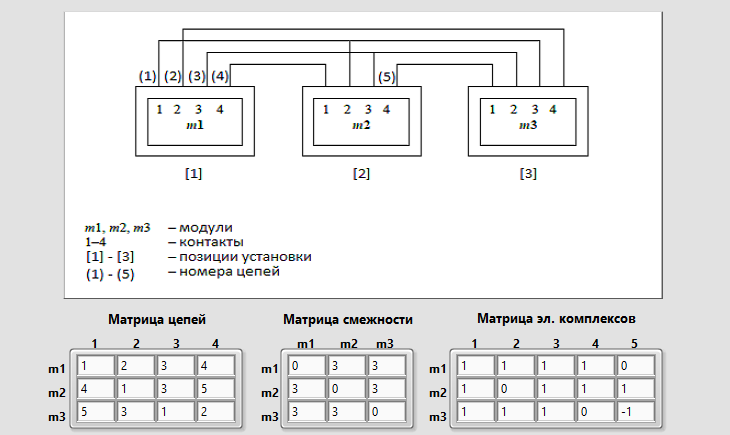
\includegraphics[width=0.7\linewidth]{image/lab_7}
	\caption{Матрица цепей Т, матрица смежности и матрица элементных комплексов}
	\label{fig:lab7}
\end{figure}


\section{Выводы по работе}

Были изучены математические модели схем и было выяснено как составлять матрицы цепей, смежности и элементных комплексов исходя из имеющейся схемы соединения элементов.

\section{Контрольные вопросы}

\begin{enumerate}
	\item Что называется математической моделью (ММ)?

Под математической моделью (ММ) конструкции, технологического процесса и его элементов понимают систему математических соотношений, описывающих с требуемой точностью изучаемый объект и его поведение в производственных условиях. При построении математических моделей используют различные математические средства описания объекта — теорию множеств, теорию графов, теорию вероятностей, математическую логику, математическое программирование, дифференциальные или интегральные уравнения и т. д.


	\item	Что называют внутренними, внешними и выходными параметрами ММ?

Внутренние параметры модели определяются характеристиками компонентов, входящих в проектируемый объект, например номиналы элементов принципиальной схемы. Если проектируемый объект содержит n элементарных компонентов, то и его математическая модель будет определяться параметрами, которые образуют вектор внутренних параметров $W = |w_1…w_n|^T$. Каждый из параметров $w^i$, в свою очередь, может быть функцией, вектором или еще более сложным математическим функционалом в зависимости от объекта проектирования.

Выходные	параметры	модели	–	это	показатели,	характеризующие

функциональные, эксплуатационные, конструкторско-технологические, экономические и другие характеристики проектируемого объекта. К таким показателям могут относиться коэффициенты передачи, масса и габариты проектируемого объекта, надежность, стоимость и т.п. Понятия внутренних и выходных параметров инвариантны, при моделировании на более сложном уровне выходные параметры могут стать внутренними и наоборот. Например, сопротивление резистора является внутренним параметром при моделировании усилительного устройства, компонентом которого он является, но это же сопротивление будет выходным параметром при моделировании самого резистора, что требуется при пленочном его исполнении. Вектор выходных параметров модели обозначают $F = |f_1…f_k|^T$.

Внешние параметры модели – это характеристики внешней по отношению к проектируемому объекту среды, а также рабочие управляющие воздействия. Вектор внешних параметров в общем случае содержит множество самых различных составляющих. К его составляющим с полным правом можно отнести все, что говорилось ранее о составляющих вектора внутренних параметров.

Будем обозначать его $Q = |q_1…q_m|^T$.

\item	Какие требования представляют к ММ объекта?


Основными требованиями, предъявляемыми к математическим моделям, являются требования адекватности, универсальности и экономичности. Модель считается адекватной, если отражает заданные свойства объекта с приемлемой точностью. Точность определяется как степень совпадения значений выходных параметров модели и объекта.

Универсальность модели определяется числом и составом учитываемых в модели внешних и выходных параметров.

Экономичность модели характеризуется затратами вычислительных ресурсов для ее реализации, а именно затратами машинного времени Тм и памяти Пм.

\item	Покажите общий вид системы уравнений для любой РЭС и дайте пояснения.

Элементы подсистем бывают простыми и сложными. Элемент называют простым, если соответствующая ему ММЭ может быть представлена в виде одного линейного уравнения, связывающего переменную типа потенциала  

и	переменную типа потока  , характеризующие состояние данного элемента. В физически однородных подсистемах различают три типа простых элементов. Это элементы емкостного, индуктивного и резистивного типов. Соответствующие им ММЭ имеют вид $C\dfrac{dU}{dt} = I; L\dfrac{dI}{dt} = U; U = RI$.
\end{enumerate}

\end{document} % конец документа